

\begin{block}{The Experiment}

Experiment setup: 

\begin{itemize}
    \item ss 
    \item 24 participants (conducted with the help of Berlin Social Science Center - WZB)
    \item Observations scenario: 2 runs (one hard and one easy), 25 rounds each
    \item Belief scenario: 1 run with 60 rounds
\end{itemize}

\begin{figure}
  \centering
    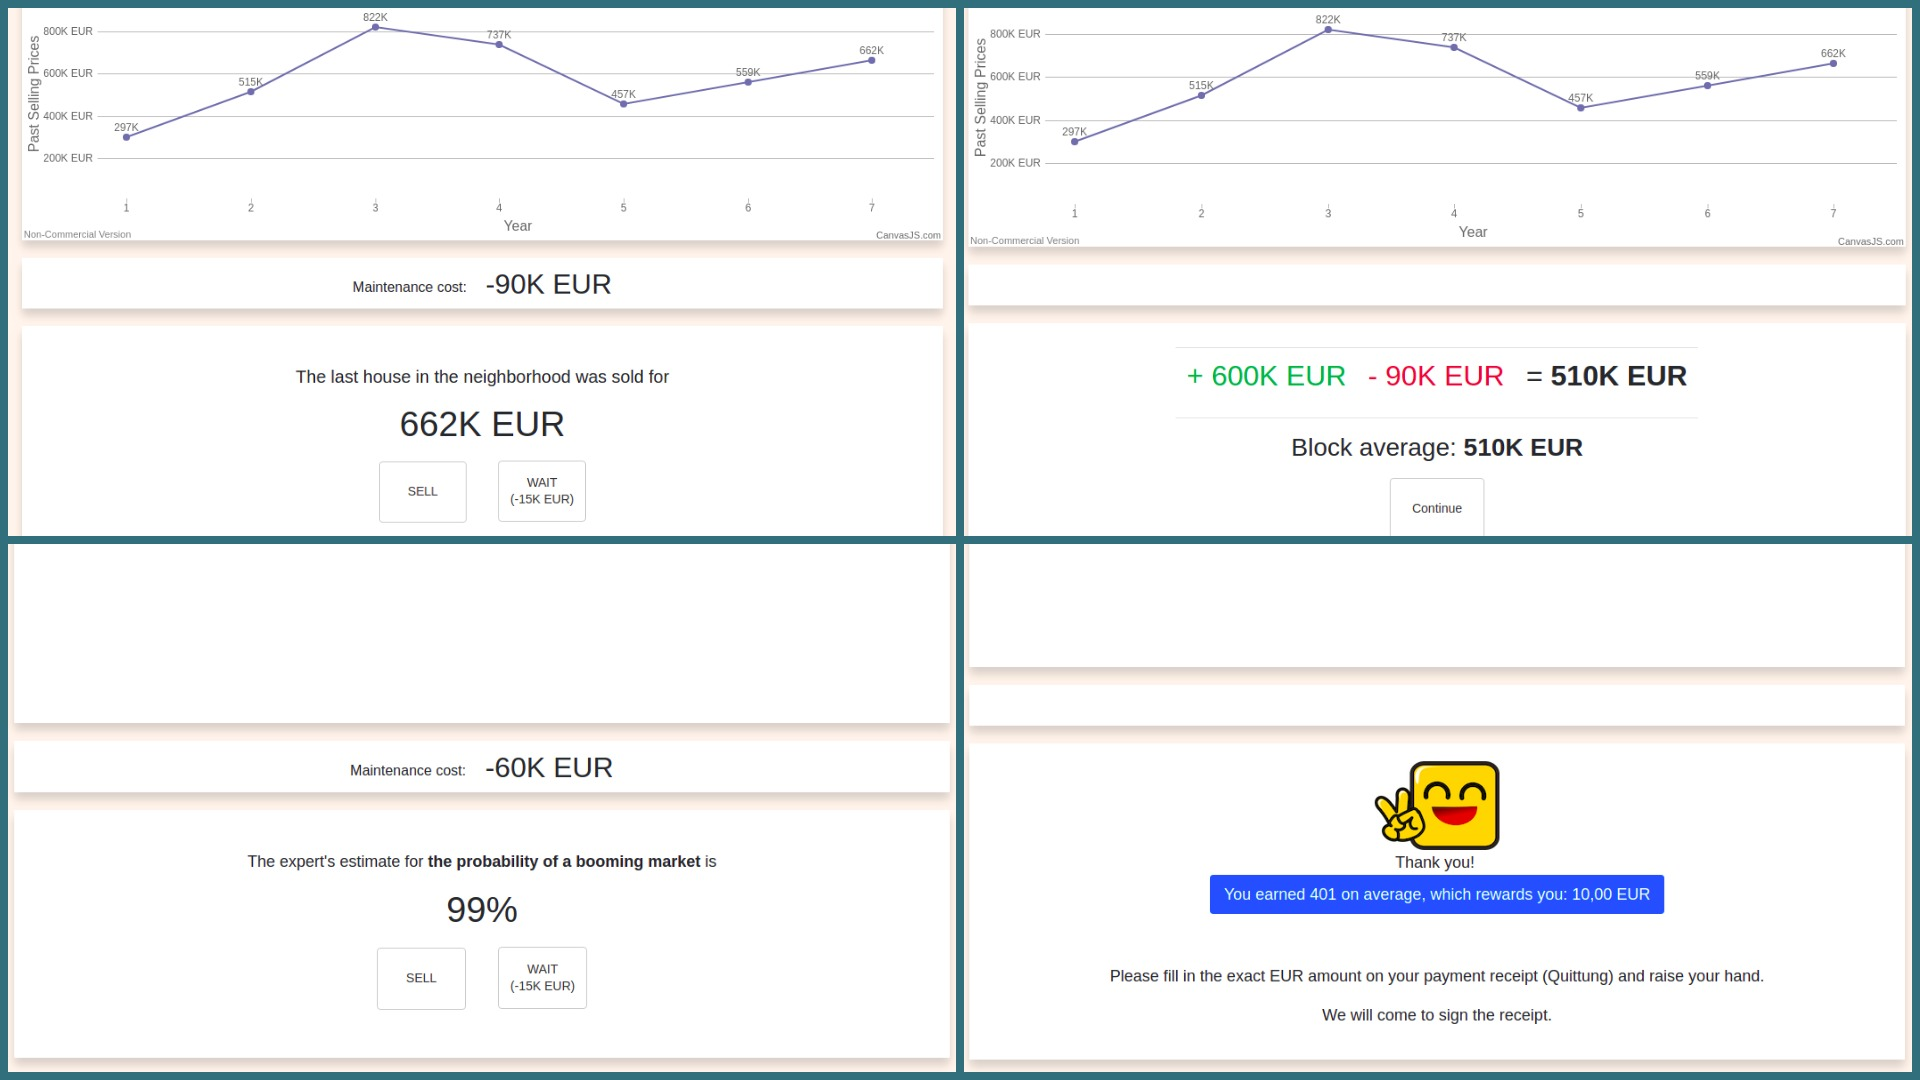
\includegraphics[width=0.9\textwidth]{img/methods/pjimage.jpg}
  \caption{Screen-shots from the software used for the experiment}
  
\end{figure}

\end{block}


\begin{block}{The Agent}

\begin{itemize}
    \item Implemented based on a value iteration solution
    \item Run artificial agents for different utility functions
\end{itemize}

\end{block}

